\documentclass[12pt]{article}

\usepackage{parskip}
\usepackage[charter]{mathdesign}
\usepackage[margin=1.2in,showframe]{geometry}
\usepackage{mathtools}

\usepackage{tikz}
%\usetikzlibrary{intersections}
\usetikzlibrary{decorations}
\usepackage{pgfplots}

%% Captions and subcaptions
\usepackage[font=footnotesize,format=plain,labelfont=bf,textfont=sl]{caption}
\usepackage[labelformat=simple,font=footnotesize,format=plain,labelfont=bf,textfont=sl]{subcaption}
%% Caption setup for figures and tables
\captionsetup[figure]{width=0.8\textwidth,format=hang,justification=centering,singlelinecheck=off,skip=2ex}
\captionsetup[table]{format=hang,justification=centering,singlelinecheck=off,skip=2ex}
\captionsetup[subfigure]{format=hang,justification=centering,singlelinecheck=off,skip=2ex}
\captionsetup[subtable]{format=hang,justification=centering,singlelinecheck=off,skip=2ex}
%% Put parens around the subfig name (a) (b) etc. Needs labelformat simple
\renewcommand\thesubfigure{(\alph{subfigure})}
\renewcommand\thesubtable{(\alph{subtable})}

\usepackage[hang,bottom]{footmisc}

\colorlet{dkgreen}{green!50!black}

\def\me{\mathrm{e}}
\def\md{\mathrm{d}}

\def\hf{0.45\textwidth}

\def\a{1.942377049}
\def\z{1.51574}
\def\q{0.663912506}

\title{Hauw's Problem\\{\large\vspace*{0.5cm} -or-\\\vspace*{0.3cm}Finding the best straight line for approaching a temperature rising curve}}
\author{Jesse op den Brouw}
\date{\today}

\begin{document}
\raggedbottom
\maketitle

\vfill
\begin{center}
In memory of colleague Hauw Khoe
\end{center}
\vfill

\begin{abstract}
\centering\noindent
This document discusses the best straight line to approach the standard curve of the temperature rise of an infinitesimal object.
\end{abstract}
\vfill

\clearpage

\section{Introduction}
Colleague Hauw Khoe has written a document for students of the XYZ\footnote{Not to be disclosed} study programme. The students had to learn about the temperature rising of an (infinitesimal) object when exposed to a sudden temperature increase. Of course he suggested a function that described the course of the temperature. Everyone knows that this function harbors an exponential function and Hauw described this in his document. However, the lectures of the said study programme felt that this description was ''too difficult'' for their students and preferred to use an approach in the form of a straight line. The students would understand this much better (Hauw suggested that this never could be the proper function, but his words were not heeded). Hauw opted for a straight line, starting at $T_{min}$, with a slope of $1/\tau$, up to $T_{max}$, after which the function further had a constant value of $T_{max}$.

\section{Heating an object}
Before we delve into the rest of the document, we should show how the temperature of an suddenly heated object elapses. The temperature of an object exposed to a sudden increase of temperature is, over time:

\begin{equation}
T_\text{offical}(t) = T_{min} + (T_{max} - T_{min})\cdot (1-\me^{-t/\tau})
\end{equation}

where $T_{min}$ is the temperature of the object before exposure and $T_{max}$ is the ultimate temperature of the object. The variable $\tau$ is the time constant. At $t=\tau$, the temperature has reached about $63\,\%$ of its final value, starting from $T_{min}$ and ending at $T_{max}$. See Figure~\ref{fig1}.

\begin{figure}[!ht]
\centering
\begin{tikzpicture}[
    declare function = { f(\x) = 1-e^(-\x); }
]
\begin{axis}[
    width=0.9\textwidth,
    height=\hf,
    ytick={0,1},
    yticklabels={$T_{min}$,$T_{max}$},
    xtick={0.01,1,4.99},
    xticklabels={0,$\tau$,$5\tau$},
    axis x line=middle,
    ymin=0.0, ymax=1.0, xmin=0.0, xmax=5.0,
]

\addplot[red] [domain=0:5,samples=101] { f(\x) };

\draw[dashed] (axis cs:0,1) -- (axis cs:5,1);

\draw[dashed] (axis cs:1,0) -- (axis cs:1,0.632);

\end{axis}
\end{tikzpicture}
\caption{Rising temperature of an object.}
\label{fig1}
\end{figure}

Now removing the occurrences of $T_{min}$ and $T_{max}$ yields only the exponential function, which is of our main concern. The function is shown in Figure~\ref{fig2}. The function will reach approximately $63\,\%$ of the end value at time $\tau$. The function is:

\begin{equation}
T(t) = 1-\me^{-t/\tau}
\end{equation}

which leaves us with a value of 0.632120559 at $t=\tau$.

\begin{figure}[!ht]
\centering
\begin{tikzpicture}[
    declare function = { f(\x) = 1-e^(-\x); }
]
\begin{axis}[
    width=0.9\textwidth,
    height=\hf,
    ytick={0,0.632,1},
%    yticklabels={$T_{min}$,$T_{max}$},
    xtick={0,1,4.99},
    xticklabels={0,$\tau$,$5\tau$},
    axis x line=middle,
    ymin=0.0, ymax=1.0, xmin=0.0, xmax=5.0,
]

\addplot[red] [domain=0:5,samples=101] { f(\x) };

\draw[dashed] (axis cs:0,1) -- (axis cs:5,1);

\draw[dashed] (axis cs:1,0) -- (axis cs:1,0.632);
\draw[dashed] (axis cs:0,0.632) -- (axis cs:1,0.632);

\end{axis}
\end{tikzpicture}
\caption{Relative rising temperature of an object.}
\label{fig2}
\end{figure}

\section{Suggested function by Hauw}
Hauw suggested a straight line function with of slope of $1/\tau$ which will reach the end value at time $\tau$. After that, the function stays at the end value. See Figure~\ref{fig3}. So Hauw's function is:

\begin{equation}
H(t) = \begin{cases}
t/\tau & \text{for } 0\leq t\leq \tau\\
1      & \text{for } \tau\leq t < \infty\\
\end{cases}
\end{equation}

\begin{figure}[!ht]
\centering
\begin{tikzpicture}[
    declare function = { f(\x) = 1-e^(-\x); }
]
\begin{axis}[
    width=0.9\textwidth,
    height=\hf,
    ytick={0,0.632,1},
%    yticklabels={$T_{min}$,$T_{max}$},
    xtick={0,1,4.99},
    xticklabels={0,$\tau$,$5\tau$},
    axis x line=middle,
    ymin=0.0, ymax=1.0, xmin=0.0, xmax=5.0,
]

\addplot[red] [domain=0:5,samples=101] { f(\x) };

\draw[dashed] (axis cs:0,1) -- (axis cs:5,1);

\draw[dashed] (axis cs:1,0) -- (axis cs:1,1);
\draw[dashed] (axis cs:0,0.632) -- (axis cs:1,0.632);

\draw[blue] (axis cs:0,0) -- (axis cs:1,1);
\draw[blue] (axis cs:1,1) -- (axis cs:5,1);

\draw [purple,decorate,decoration={brace,amplitude=10pt,mirror},xshift=1] (axis cs: 1,0.632) -- (axis cs:1,1) node[midway,xshift=20] {$\Delta y$};

\end{axis}
\end{tikzpicture}
\caption{Hauw's function $H(t)$ and relative rising temperature of an object $T(t)$.}
\label{fig3}
\end{figure}

Obviously, there is a discrepancy between Hauw's function and the real function as shown in Figure~\ref{fig3}. The maximum discrepancy is denoted by $\Delta y$ and is

\begin{equation}
1 - (1-\me^{-1}) = 0.367879441 \qquad (t=\tau)
\end{equation}

\begin{figure}[!ht]
\centering
\begin{tikzpicture}[
    declare function = { f(\x) = 1-e^(-\x); }
]
\begin{axis}[
    width=0.9\textwidth,
    height=\hf,
    ytick={0,0.368,0.5},
%    yticklabels={$T_{min}$,$T_{max}$},
    xtick={0,1,4.99},
    xticklabels={0,$\tau$,$5\tau$},
    axis x line=middle,
    ymin=0.0, ymax=0.5, xmin=0.0, xmax=5.0,
]

\addplot[red] [domain=0:1,samples=101] { \x-f(\x) };
\addplot[red] [domain=1:5,samples=101] { 1-f(\x) };

\draw[dashed] (axis cs:1,0) -- (axis cs:1,0.368);
\draw[dashed] (axis cs:1,0.368) -- (axis cs:0,0.368);

\draw [purple,decorate,decoration={brace,amplitude=10pt,mirror},xshift=1] (axis cs: 1,0) -- (axis cs:1,0.368) node[midway,xshift=20] {$\Delta y$};

\end{axis}
\end{tikzpicture}
\caption{Difference between Hauw's function $H(t)$ and relative rising of the temperature of an object $T(t)$.}
\label{fig4}
\end{figure}

The deviation between Hauw's function and the relative rising of the temperature can be seen in Figure~\ref{fig4}. As can be seen, the maximun deviation is at $t=\tau$.

\section{Proposed function}
We propose a moderation of Hauw's function. We introduce a variable $\alpha$ to control the slope of the straight line. Note that $\tau$ is constant for a certain object.

\begin{equation}
P(t) = \begin{cases}
t/\alpha\tau & \text{for } 0\leq t\leq \alpha\tau\\
1      & \text{for } \alpha\tau\leq t < \infty\\
\end{cases}
\end{equation}

Note that is a non-continuous function.
Hauw's function $H(t)$, the rising temperature function $T(t)$ and the proposed function $P(t)$ are shown in Figure~\ref{fig5}. Note that $P(t)$ and $T(t)$ intersect at $t=z\tau$. Note that $z$ depends on $\alpha$.

\begin{figure}[!ht]
\centering
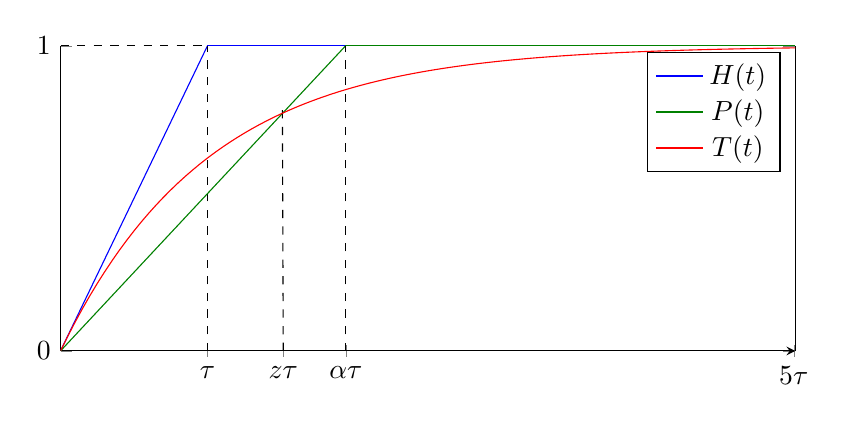
\begin{tikzpicture}[
    declare function = { T(\x) = 1-e^(-\x); P(\x) = 1.0/1.94*\x; }
]
\begin{axis}[
    width=0.9\textwidth,
    height=\hf,
    ytick={0,1},
    xtick={0,1,\z,\a,4.99},
    xticklabels={0,$\tau$,$z\tau$,$\alpha\tau$,$5\tau$},
    axis x line=middle,
    ymin=0.0, ymax=1.0, xmin=0.0, xmax=5.0,
    legend entries={$H(t)$,$P(t)$,$T(t)$},
]

% The ending value
\draw[dashed,black] (axis cs:0,1) -- (axis cs:5,1);

% Function based on tau
\addplot[blue] [domain=0:1] { \x };
\draw[blue] (axis cs:1,1) -- (axis cs:5,1);
\draw[dashed] (axis cs:1,0) -- (axis cs:1,1);

% Function based on alpha*tau
\addplot[dkgreen] [domain=0:\a] { P(\x) };
\draw[dkgreen] (axis cs:\a,1) -- (axis cs:5,1);
\draw[dashed] (axis cs:\a,0) -- (axis cs:\a,1);

% Function based on z
\draw[dashed] (axis cs:\z,0) -- (axis cs:1.51,0.79);

\addplot[red] [domain=0:5,samples=101] { T(\x) };
\end{axis}
\end{tikzpicture}
\caption{Showing Hauw's function $H(t)$ (blue), temperature rising function $T(t)$ (red) and the proposed function $P(t)$ (green).}
\label{fig5}
\end{figure}

Obviously, we can see that $\alpha \geq 1$ since $\alpha=1$ for $P(t)$, $P(t)$ is equal to $H(t)$. We need to find an $\alpha$ where the difference between $P(t)$ and $T(t)$ is minimal. We denote this function $G(t)$. This difference is shown in Figure~\ref{fig6}. So:

\begin{equation}
G(t) = P(t) - T(t)
\end{equation}

\begin{figure}[!ht]
\centering
\begin{tikzpicture}[
    declare function = { T(\x) = 1-e^(-\x); P(\x) = 1.0/\a*\x; }
]
\begin{axis}[
    width=0.9\textwidth,
    height=\hf,
    ytick={-0.25,0.25},
    xtick={0,\q,1,\z,\a,4.99},
    xticklabels={0,$q\tau$,$\tau$,$z\tau$,$\alpha\tau$,$5\tau$},
    axis x line=middle,
    ymin=-0.25, ymax=0.25, xmin=0.0, xmax=5.0,
]

\addplot[red] [domain=0:\a] { P(\x)-T(\x) };
\addplot[red] [domain=\a:5] { 1-T(\x) };

\draw[dashed] (axis cs:0,-0.143362764) -- (axis cs:\q,-0.143362764);
\draw[dashed] (axis cs:0,0.143362764) -- (axis cs:\a,0.143362764);
\end{axis}
\end{tikzpicture}
\caption{Function $G(t)$, the difference between $P(t)$ and $T(t)$.}
\label{fig6}
\end{figure}

%Now increasing $\alpha$ will shift $t=\alpha\tau$ to the right and will increase the $y$ value at this point.
%Based

We split $G(t)$ in two helper functions to describe the flow:

\begin{align}
G_1(t) &= P(t)-T(t) = t/\alpha\tau - (1-\me^{-t/\tau}) && 0 \leq t \leq \alpha\tau \\
G_2(t) &= P(t)-T(t) = 1 - (1-\me^{-t/\tau}) && \alpha\tau \leq t < \infty
\end{align}

For function $G_1(t)$ there is a minimin at $t=q\tau$. We need to find this minimum. So we have:

\begin{equation}
\frac{\md G_1(t)}{\md t} = 0 \quad\longrightarrow\quad \frac{1}{\alpha\tau} - \frac{\me^{-t/\tau}}{\tau} = 0 \quad \longrightarrow \quad t = \tau \ln \alpha
\end{equation}

so $q=\ln\alpha$. Now we fill in this result into $G_1(t)$ we get:

\begin{equation}
G_1(t) \big|_{t=\tau\ln\alpha} = \frac{1}{\alpha}\ln\alpha + \frac{1}{\alpha} - 1
\end{equation}

Note that this value is \emph{negative} for $\alpha>1$. Also note $\tau$ is disappeared in this function. So the point of the lowest $y$ value of $G_1(t)$ solely depends on $\alpha$.

The maximum value of $G(t)$ is where $G_1(t)$ meets $G_2(t)$. This is by definition at $t=\alpha\tau$. We could use either function, because the result is the same:

\begin{equation}
G_1(t)\big|_{t=\alpha\tau} = G_2(t)\big|_{t=\alpha\tau}
\end{equation}

Using $G_2(t)$ we find:

\begin{equation}
G_2(t)\big|_{t=\alpha\tau} = 1 - (1-\me^{-t/\tau})\big|_{t=\alpha\tau} = \me^{-\alpha\tau/\tau} = \me^{-\alpha}
\end{equation}

Note that this value is \emph{positive}. Also note that $\tau$ has disappeared in this function.


Now the optimum value for $\alpha$ is when the deviations of $G_1(t)$ equals $G_2(t)$ so neither deviation is greater or smaller than the other. Because the maximum of $G_1(t)$ is negative, we have to change the sign. Changing the sign of $G_1(t)$ we find:

\begin{equation}
1 - \frac{1}{\alpha} - \frac{1}{\alpha}\ln\alpha = \me^{-\alpha}
\end{equation}

This non-linear function can only be solved by approximation, so we get:

\begin{equation}
\begin{split}
\alpha_1 = 0.42663268550049 \\
\alpha_2 = 1.94237704854534
\end{split}
\end{equation}

The value of $\alpha_1$ is not applicable because $\alpha\geq1$. So the only correct result is $\alpha_2$. Using this value we can calculate $z$ and $q$ (see Figure~\ref{fig6}).

For $z$ we find:

\begin{equation}
\begin{split}
z &\longrightarrow \left\{P(t) = T(t)\right\}\big|_{\substack{\alpha=\alpha_2 \\ t=z\tau}} \\
  &\longrightarrow \frac{z\tau}{\alpha_2\tau} = 1 - \me^{-z\tau/\tau}\\
  &\longrightarrow \frac{z}{\alpha_2} = 1 - \me^{-z} \\
  &\longrightarrow z = 1.51574
\end{split}
\end{equation}

and for $q$ we find:

\begin{equation}
q = \ln\alpha_2 = 0.663912506
\end{equation}

For the maximum deviation, we find using $G_2(t)$:

\begin{equation}
\delta = e^{-\alpha_2} = 0.143362764
\end{equation}

\section{Conclusion}

The best approach for the function with the minimum deviation of $P(t)$ from $T(t)$ is:

\begin{equation}
P(T) = \begin{cases}
\frac{1}{1.94237704854534\tau}\cdot t & \text{for } 0 \leq t \leq 1.94237704854534\tau \\
1 & \text{for } 1.94237704854534\tau \leq t \leq \infty
\end{cases}
\end{equation}

A good approximation would be to set the constant in the denominator to 2 for easy computations.

\begin{equation}
P(T) = \begin{cases}
\frac{1}{2\tau}\cdot t & \text{for } 0 \leq t \leq 2\tau \\
1 & \text{for } 2\tau \leq t \leq \infty
\end{cases}
\end{equation}



\end{document}